\subsection{Virtual Address Translation}
\label{virtual-memory-case-study}

% Point of this paragraph: We need a framework to co-design accelerators together with the virtual memory system.
With an RTL-level implementation that supports virtual memory, users can co-design their own virtual address translation schemes based on their accelerator and SoC configuration. Prior works in virtual address translation for DNN accelerators have proposed very different translation schemes, from NeuMMU~\cite{neummu-asplos2020}, which calls for a highly parallel address-translation system with 128 page-table walkers (PTWs), to Cong et al.~\cite{address-trans-cong-hpca2017}, who recommend a more modest two-level TLB hierarchy, with the host CPU's default PTW co-opted to serve requests by the accelerator. This lack of convergence in the prior literature motivates a platform that allows co-design and design-space exploration of the accelerator SoC together with its virtual address translation system, for both hardware designers and researchers. Fortunately, with Gemmini, we can iterate over a variety of address translation schemes as we tune the accelerator and SoC.

% Point of this paragraph: Describe our experimental setup
To demonstrate, we configure Gemmini to produce a two-level TLB cache, with one private TLB for the accelerator, and one larger shared TLB at the L2 cache that the private TLB falls back on when it misses. Our design includes only one PTW, shared by both the CPU and the accelerator, which is suitable for low-power devices. We configure the accelerator for low-power edge devices, with a 16-by-16 systolic mesh and a 256 KB scratchpad. As shown in Figure~\ref{fig:tlb_wait_cycles}, we iterate over a variety of TLB sizes to find the design that best balances TLB overhead and overall performance, including over a design point where the shared L2 TLB has zero entries.

% Point of this paragraph: The private TLB gives you much more bang-for-your-buck than the L2 TLB.
Figure~\ref{fig:tlb_wait_cycles} demonstrates that the private accelerator TLB has a far greater impact on end-to-end performance than the much larger shared L2 TLB. Increasing the private TLB size from just four to 16 improves performance by up to 11\%. However, adding even 512 entries to the L2 TLB never improves performance by more than 8\%. This is because our workloads exhibit high page locality; even with tiled workloads, our private TLB's hit rate remained above 84\%, even with the smallest TLB sizes we evaluated. In fact, we found that 87\% of consecutive \textit{read} TLB requests, and 83\% of consecutive \textit{write} TLB requests, were made to the same page number, demonstrating high page locality. However, because reads and writes were overlapped, read and write operations could evict each other's recent TLB entries.

\begin{figure}
    \centering
    \begin{subfigure}[t]{0.439\linewidth}
        \centering
        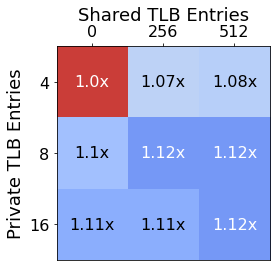
\includegraphics[width=\linewidth]{fig/tlb_entries.png}
        \caption{Without filter registers.}
        \label{fig:tlb_wait_cycles}
    \end{subfigure}
    \hfill
    \begin{subfigure}[t]{0.439\linewidth}
        \centering
        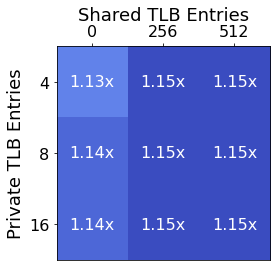
\includegraphics[width=\linewidth]{fig/tlb_entries_with_filter.png}
        \caption{With filter registers.}
        \label{fig:tlb_wait_cycles_with_filter}
    \end{subfigure}
    \caption{Normalized performance of ResNet50 inference on Gemmini-generated accelerator with different private and shared TLB sizes.}
    \vspace{-0.2in}
\end{figure}

% Point of this paragraph: On top of tuning the TLB sizes, we can make small optimizations to the virtual address translation system.
Although tuning TLB sizes improves hit rates, our private TLB hit latency in the tests shown in Figure~\ref{fig:tlb_wait_cycles} was still several cycles long. Fortunately, using the Gemmini platform, we were able to implement a simple optimization: a single register that caches the last TLB hit for read operations, and another register that caches TLB hits for write operations. These two registers allow the DMA to ``skip'' the TLB request if two consecutive requests are made to the same virtual page number, and help reduce the possibility of read-write contention over the TLB. These ``filter registers'' reduce the TLB hit latency to 0 cycles for consecutive accesses to the same page. As Figure~\ref{fig:tlb_wait_cycles_with_filter} shows, this low-cost optimization significantly improves our end-to-end performance, especially for small private TLB sizes. Due to our high TLB hit rate and low TLB hit penalty, we found that a very small 4-entry private TLB equipped with filter registers, but without an expensive shared L2 TLB, achieved only 2\% less than the maximum performance recorded. With such a configuration, the private TLB hit rate (including hits on the filter registers) reached 90\% and further increases to either TLB's size improved performance by less than 2\%, even if hundreds of new TLB entries were added.
% the total number of cycles spent by the DMA waiting for a TLB response only reached \textcolor{red}{X\%} of the total end-to-end runtime, showing that the virtual address translation scheme was no longer a primary performance bottleneck.

Using Gemmini, we have demonstrated that a modest virtual address translation system, with very small private TLBs, a single page-table-walker, and two low-cost filter registers for the TLB, can achieve near maximum performance for low-power edge devices. Gemmini is designed to enable such co-design of the SoC and its various components, such as its virtual address translation system.
